\documentclass{article}

% if you need to pass options to natbib, use, e.g.:
%     \PassOptionsToPackage{numbers, compress}{natbib}
% before loading neurips_2024


% ready for submission
\usepackage[final]{neurips_2024}


% to compile a preprint version, e.g., for submission to arXiv, add add the
% [preprint] option:
%     \usepackage[preprint]{neurips_2024}


% to compile a camera-ready version, add the [final] option, e.g.:
%     \usepackage[final]{neurips_2024}


% to avoid loading the natbib package, add option nonatbib:
%    \usepackage[nonatbib]{neurips_2024}


\usepackage[utf8]{inputenc} % allow utf-8 input
\usepackage[T1]{fontenc}    % use 8-bit T1 fonts
\usepackage{hyperref}       % hyperlinks
\usepackage{url}            % simple URL typesetting
\usepackage{booktabs}       % professional-quality tables
\usepackage{amsfonts}       % blackboard math symbols
\usepackage{nicefrac}       % compact symbols for 1/2, etc.
\usepackage{microtype}      % microtypography
\usepackage{xcolor}         % colors
\usepackage{amsmath}
\usepackage{amsthm}
\usepackage{mathrsfs}
\usepackage{graphicx}
\usepackage{caption}
\usepackage{float}


\newtheorem{theorem}{Theorem}
\newtheorem{definition}{Definition}
\newtheorem{remark}{Remark}
\newtheorem{example}{Example}
\newtheorem{proposition}{Proposition}

\title{Modeling Neural Random Field through Operator-based Diffusion}


% The \author macro works with any number of authors. There are two commands
% used to separate the names and addresses of multiple authors: \And and \AND.
%
% Using \And between authors leaves it to LaTeX to determine where to break the
% lines. Using \AND forces a line break at that point. So, if LaTeX puts 3 of 4
% authors names on the first line, and the last on the second line, try using
% \AND instead of \And before the third author name.


\author{%
    Guanyu Chen \\
    College of Integrated Circuits\\
    Zhejiang Uinversity\\
    Hangzhou, Zhejiang\\
    \texttt{guanyu@zju.edu.cn} 
}


\begin{document}


\maketitle


\begin{abstract}

\end{abstract}


\section{Introduction}
\begin{definition}
    Random field $\mathcal{M}(x, \omega)$, where $x\in D$ and $\omega \in \Omega$, is defined as:
\begin{equation}
    \begin{aligned}
        & \mathcal{M}(x, \cdot) \text{ is a random variable defined on the probability space } (\Omega, \mathcal{F}, P),\\
        & \mathcal{M}(\cdot, \omega) \text{ is a deterministic function of } x.
    \end{aligned}
\end{equation}
\end{definition}
In fact, a random field is an infinite-dimensional distribution over functions, and can therefore be understood as a Function Distribution/Function Space. 
Classical methods to simulate random field are based on polynomial chaos expansion \ref{PCE} and Karhunen-Loeve expansion \ref{KLE}, See \cite{Lord_Powell_Shardlow_2014}.
Random field can be regarded as a Hilbert space($L^2(\Omega, H)$)-valued random variable.
\begin{definition}[$L^p(\Omega, H)$ space]
  Let $(\Omega, \mathcal{F}, \mathbb{P})$ be a probability space and $H$ is a Hilbert space with norm $\|\cdot\|$. Then $\mathcal{L}^p(\Omega, H)$ with $1\leq p<\infty$ is the space
  of H-valued $\mathcal{F}$-measurable random vaiables $X:\Omega\rightarrow H$ with $\mathbf{E}[\|X\|^p]<\infty$ and a Banach space with norm:
  \begin{equation}
      \|X\|_{\mathcal{L}^p(\Omega, H)}:=\left(\int_\Omega \|X(\omega)\|^pdP(\omega)\right)^{\frac{1}{p}}=\mathbf{E}[\|X\|^p]^{\frac{1}{p}}
  \end{equation}
\end{definition}
Then we can define the inner product: 
\begin{equation}
  \langle X, Y\rangle_{\mathcal{L}^2(\Omega, H)}:=\int_\Omega \langle X(\omega), Y(\omega)\rangle_H dP(\omega)
\end{equation}

\begin{definition}[uncorrelated, covariance operator]
  Let $H$ be a Hilbert space. A linear operator $\mathcal{C}:H\rightarrow H$ is the covariance of $H$-valued random variables $X$ and $Y$ if 
  \begin{equation}
      \langle\mathcal{C}_{XY}\phi, \psi\rangle_H = \operatorname{Cov}\left(\langle X, \phi\rangle_H, \langle Y, \psi\rangle_H\right), \forall \phi, \psi \in H
  \end{equation}
\end{definition}
The covariance operator plays a special role as it characterizes the properties of the random field, like regularity and smoothness.

\begin{example}[$H = \mathbb{R}^d$]
  In finite dimensional case $H = \mathbb{R}^d$, the covariance matrix conincides with the covariance operator. 
  \begin{equation}
      \begin{aligned}
          &\operatorname{Cov}\left(\langle X, \phi\rangle, \langle Y, \psi\rangle\right) 
          = \operatorname{Cov}\left(\phi^T X, \psi^T Y\right)\\
          =&\mathbf{E}\left[\phi^T(X-\mu_X)(Y-\mu_Y)^T\psi\right] 
          = \phi^T\mathbf{E}\left[(X-\mu_X)(Y-\mu_Y)^T\right]\psi\\
          =&\phi^T Cov(X, Y)\psi = \langle C_{XY}\phi, \psi\rangle
      \end{aligned}
  \end{equation}
\end{example}

\begin{example}[X=Y]
  When $X = Y$ noted as $u(x, \omega)\in H$, the covariance operator:
  The covariance operator $\mathcal{C}$ can be defined as:
  \begin{equation}
    \begin{aligned}
      &Cov\left(\langle u, \phi\rangle_{H}, \langle u, \psi\rangle_{H}\right)\\
      =&\mathbb{E}_m\left[\langle u, \phi\rangle_{H}\langle u, \psi\rangle_{H}\right]\\
      =& \int_{H}\langle u, \phi\rangle_{H}\langle u, \psi\rangle_{H} m(du)\\
      =&\int_D\left(\int_D Cov(u(x), u(y)) \phi(x) dx \right) \psi(y) dy\\
      =& \langle\mathcal{C}_u\phi, \psi\rangle_{H} 
    \end{aligned}
   \end{equation}
  So that for $\forall x\in D$,
  \begin{equation}
  (\mathcal{C}_u\phi)(x) = \int_D Cov(u(x), u(y)) \phi(y) dy
  \end{equation}
  That is any $L^2(D)$-valued random variable $u(x)$ can defines a R.F. with $\mu(x)$ and $C(x, y)$ equal to the integral kernel of $\mathcal{C}$.
  The measure $m$ is called probability measure.
\end{example}

\begin{definition}[Trace class]\label{thmtraceclass}
  For random field $u(x,\omega)$ with the covariance operator $\mathcal{C}$, suppose $\mathcal{C}$ is trace class with eigenpairs $(\lambda_i, \phi_i)$, 
  then the second moment of $u(x, \omega)$ is given by:
  \begin{equation}
    \mathbf{E}[\|u(x, \omega)\|^2_H] = \sum_{i=1}^{\infty} \lambda_i\leq \infty
  \end{equation}
\end{definition}

\begin{definition}[H-valued Gaussian random variable]
  Let $H$ be a Hilbert space. An H-valued random variable $u(x, \omega)$ is Gaussian if 
  $\langle u(x, \omega), \phi\rangle_H$ is a real-valued Gaussian random variable for all $\phi \in H$.
  Here the real-valued Gaussian Random Variable is defined as:
  \begin{equation}
    \langle u, \phi\rangle_H \sim N(\langle \mu, \phi\rangle_H, \langle \mathcal{C}_u\phi, \phi\rangle_H)
  \end{equation}
  This actually defines the Gaussian Measure $m$ on $H$: $u\sim N(\mu, \mathcal{C}_u):= m$. 
  The covariance operator of $u$ is the symmetric, positive-definite operator $\mathcal{C}_u : H \rightarrow H$.
\end{definition}

\begin{proposition}
  If $u(x, \omega)$ is a Gaussian random field, then $\mathcal{C}_u$ is trace class. 
  Reversely, if $\mathcal{C}_u$ is a positive, symmetric, trace class operator in H, then there exists a Gasussian measure $m=N(0, \mathcal{C}_u)$ on H.
\end{proposition}

Since we consider infinite dimensional case, unlike finite dimensions, not all translations preserve the measure. 
We need to cansider those directions in $H$ along which translating a Gaussian measure does not change its essential nature (i.e., keeps it equivalent). 
First we have some definitions:
\begin{definition}
  Let $m_1, m_2$ be two measures on $H$.
  \begin{itemize}
    \item $m_1 \ll m_2$ means measure $m_1$ is absoutely continuous respect to $m_2$: if $m_1(A) = 0$ for all $A$ s.t. $m_2(A) = 0$. 
     This means that the support of $m_1$ is a subset of the support of $m_2$.
    \item If $m_1 \ll m_2, m_2 \ll m_1$, $m_1, m_2$ are said to be equivalent $m_1 \sim m_2$.
    \item If there exists a measurable set $A$ s.t. $m_1(A) = 0$ and $m_2(A^c) =1$, then $m_1, m_2$ are singular $m_1 \perp m_2$. 
  \end{itemize}
\end{definition}

\begin{theorem}[Radon-Nikodym Theorem]
  Let $S = (H,\mathcal{B}(H))$ be a measurable space. $m_1, m_2$ are two $\sigma$-finite measures on $S$. \
  if $m_1 \ll m_2$, then there exists a measurable function $f:H\rightarrow [0, \infty)$ s.t. $m_1(A) = \int_A f dm_2, \forall A \in \mathcal{B}(H)$.
  The function $f$ is called the Radon-Nikodym derivative of $m_1$ with respect to $m_2$ and is denoted by $f = \frac{dm_1}{dm_2}$.
\end{theorem}

\begin{example}
  In finite dimensional case, the Radon-Nikodym derivative is the probability density function. 
  Like $m_2$ is the Lebesgue measure, $m_1(dx) = p(x)dx$, then the Radon-Nikodym derivative is the probability density function $p(x)$. 
\end{example}

\begin{definition}[KL-divergence]
  The KL-divergence is actually related to the Radon-Nikodym derivative: if $m_1 \ll m_2$, then:
  \begin{equation}
    \operatorname{KL}(m_1||m_2) = \int_H \log\left(\frac{dm_1}{dm_2}(x)\right) dm_1(x) 
    = \int_H \log\left(f(x)\right) f(x)dm_2(x)
  \end{equation}
  This is the KL divergence between measures. We define the Radon-Nikodym derivative to be infinite if $m_1 \not\ll m_2$.
  So for $H=\mathbb{R}^d, dm_1 = p_1(x)dx, dm_2 = p_2(x)dx$, the KL-divergence can be written as:
  \begin{equation}
    \operatorname{KL}(m_1||m_2) = \int_{\mathbb{R}^d} \log\left(\frac{p_1(x)}{p_2(x)}\right) p_1(x) dx
  \end{equation}
  The Radon-Nikodym derivative captures local density ratios, and the KL divergence is their global average.
\end{definition}

Unlike the finite dimensional case, there is no natural Brownian Motion process in infinite dimensions. 
Here is why: For example, the space time white noise $W_t$ is defined on $H=L^2([0, 1])$, but it doesn't take values in $H$ a.s.
Since the white noise has covariance operator $I$, it is not trace class in $H$. 
So for Hilbert space $H$, we need to define the Brownian Motion process on $H$ by using the Cameron-Martin space $U$.
% In Cameron-Martin space, the white noise is a trace class operator.
In other words, if we want to define the Diffusion Process on infinite dimensional space, 
we need to consider the direction in $H$ along which translating a measure preserves the absolutely continuity.


\begin{definition}[Cameron-Martin Space]
The Cameron-Martin space $U$ is defined as:
\begin{equation}
  U:=\{h\in H| m_h\ll m\},m_h(A)=T_h^\#m(A):= m(A-h),\forall A \in \mathcal{B}(H)
\end{equation} 
where $T_h$ is the translation operator: $T_h(u)=u + h$, $T_h^\#m$ is the push-forward measure of $m$ by $T_h$, 
\end{definition}
So the Cameron-Martin space $U$ is more regular than the original space $H$.

\begin{theorem}[Cameron-Martin Theorem]
  For $m=N(0, \mathcal{C})$, we have:
  \begin{equation}
    m_h\sim m \text{ if and only if } h\in \mathcal{C}^\frac{1}{2}H:=U
  \end{equation}
  Since $\mathcal{C}^{-1}$ is unbounded, $U$ is a proper subspace of $U = \mathcal{C}^{1/2}H$.
  The inner product is defined as:
\begin{equation}
  \langle \phi, \psi\rangle_U = \langle \mathcal{C}^{-1/2}\phi, \mathcal{C}^{-1/2}\psi\rangle_H
\end{equation}
\end{theorem}

This can be generalized to general Gaussian measure cases:
\begin{theorem}[Feldman-Hajek Theorem\cite{Prato_Zabczyk_2014}]
  The following statements hold:\\
  1. $m_1 = N(\mu_1, \mathcal{C}_1), m_2 = N(\mu_2, \mathcal{C}_2)$ are either singular or equivalent.\\
  2. They are equivalent if and only if 
  \begin{itemize}
      \item $\mathcal{C}_1^{1/2}(H) = \mathcal{C}_2^{1/2}(H)=H_0$, $\mu_1 - \mu_2 \in H_0$
      \item $(\mathcal{C}_1^{-1/2}\mathcal{C}_2^{1/2})(\mathcal{C}_1^{-1/2}\mathcal{C}_2^{1/2})^*-I$ is a Hilbert-Schmidt operator.
  \end{itemize}
  Specifically, if $\mathcal{C}_1=\mathcal{C}_2=\mathcal{C}$, we have the Radon Nikodym derivative:
  \begin{equation} 
    \frac{dm_1}{dm_2}(u) = \exp{\left(\langle \mu_1 - \mu_2, \mathcal{C}^{-1}(u - \mu_2) \rangle_H - \frac{1}{2}\|\mathcal{C}^{-1/2}(\mu_1 - \mu_2)\|^2_H\right)}
  \end{equation}
  Therefore, the KL divergence between $m_1$ and $m_2$ is:
  \begin{equation}
    \operatorname{KL}[m_1|m_2] = \frac{1}{2}\left(\|\Delta\mu, C^{-1}\Delta \mu\|^2_H\right)
  \end{equation}
\end{theorem}
Meanwhile, for Gaussian measure $m=N(\mu, \mathcal{C})$, we have the characteristic functional:
\begin{equation}
  \hat{m}(\lambda) = \int_H e^{i\langle \lambda, u\rangle_H} m(du) = e^{i\langle \lambda, \mu\rangle_H-\frac{1}{2}\langle \lambda, \mathcal{C}\lambda\rangle_H}, \qquad \lambda\in H
\end{equation}

First we assume define the Cylindrical Wiener Process $\hat{W}_t$ on $H$, but it does not take values in $H$ cause $I$ is not a trace class.
Here we suppose $\hat{W}_t$ is $H_1$-valued:
\begin{equation}
  \hat{W}_t = \sum_{i=1}^{\infty} \beta_i(t) \phi_i
\end{equation}
where $\beta_i(t)$ are independent standart Brownian motions and $\phi_i$ are the eigenbasis of $H$.
Normally, we can define the $\mathcal{C}$-Wiener Process on $H$ as:
\begin{definition}[$\mathcal{C}$-Wiener Process]
  A H-valued process $W_t$ is called $\mathcal{C}$-Wiener process if:
  1. $W_0 = 0$
  2. $W_t$ has continuous trajectories: $\mathbb{R}^+\rightarrow H$
  3. $W_t$ has independent Gaussian increments: $m(W_t - W_s) = N(0, (t-s)\mathcal{C})$
\end{definition}
Therefore by applying the covariance operator $\mathcal{C}$ to cylindrical Wiener Process $\hat{W}_t$, we can define the $H$-valued $\mathcal{C}$-Wiener process $W_t$ as:
\begin{equation}
  W_t = \sum_{i=1}^{\infty} \sqrt{\lambda_i} \beta_i(t) \phi_i = \mathcal{C}^{1/2}\hat{W}_t
\end{equation}
where $\lambda_i$ are the eigenvalues of $\mathcal{C}$. 
So $H$ is actually the Cameron-Matin space of $H_1$.

To sum up, in infinite dimensional diffusion model, suppose we have $u\sim m_0, \eta\sim m_1$, where $m_0$ is the initial measure and $m_1$ is the target measure, all defined on $H$.
In the diffusion process, we add noise process $\eta$ to $u$, getting $v = u + \eta$. Then $v\sim \nu=m_0 * m_1$. Here we need to do some assumptions on measure $m_0$ and $m_1$: 
$m_0$ needs to be supported on the Cameron-Martin space $U$ of $m_1$, that is $m_0 \ll m_1$, $m_0$ should be more regular than $m_1$. 
Only in this way, we can define the Radon-Nikodym derivative of $\nu$ with respect to $m_1$, and the perturbed measure $\nu$ is equivalent to $m_1$.

Normally, to guarantee the diffusion progress, we have two choices: 1. The support of $m_{data}$ is contained in Camaron-Martin space of $N(0, \mathcal{C}_{data})$ 2. Choose a large space $K$, s.t. the support of $m_{data}$ and $N(0, \mathcal{C})$ are supported on $K$.

\begin{definition}[Problem Setting]
  Assume we have $H$-valued Random Fields $\mathcal{M(x, \omega)}$ defined on $(H, \mathcal{B}(H), m)$ and $\mathcal{N(x, \omega)}$ defined on $(H, \mathcal{B}(H), m_0)$, where $m_0$ is the initial probability measure.
  We consider the following problem: 
  \begin{itemize}
    \item How to build a generative model to sample from the unknown measure $m_0$? 
    Conversly, given the target measure and initial measure, how to build the push forward operator $\mathcal{L}$?
    \item Given the initial measure $m_0$ and the push forward operator $\mathcal{L}$, what is the measure $m_t, \forall t\in [0, 1]$?
  \end{itemize}
\end{definition}

\section{Related Work}
Some references: \cite{whittle1954stationary, carrizo2022general, lindgren2020diffusion, sigrist2015stochastic, bolin2020rational, Porcu2023}

\cite{dupont2022generativemodelsdistributionsfunctions}
\cite{mittal2022pointsfunctionsinfinitedimensionalrepresentations}

\paragraph{Diffusion model in function space}
Kerrigan et al. \cite{kerrigan2023diffusiongenerativemodelsinfinite} first studied the diffusion model in function space and KL approximation. 
This work can be viewed as a generalization of DDPM in function space. They first combine the diffusion model with neural operators.
But they only consider the Gaussian measure and do discretiztion on function space to which the KL approximation is sensitive.
In DDO\cite{lim2025scorebaseddiffusionmodelsfunction}, Lim et all. offered an alternative viewpoint with the score defined as a logarithmic derivative of a perturbed measure and sampling done by a Langevin process and its annealed version.
They generate the notion of score and denoising score matching to infinite dimensions.
In IDDM\cite{JMLR:v25:23-1271}, Pidstrigach et all. formulate the diffusion model algorithm directly on infinitedimensional spaces, and proves that this formulation is well-posed and satisfies crucial theoretical guarantees.
They discussed three challenges in infinite dimensional diffusion model: 1. how to define the noise function $W_t$ 2. how to define the score function and the loss function 3. how to sample from measure space.
All these challenges are related to the data distribution. They provide a theoretical framework for infinite dimensional diffusion model on how to solve these challenges.
The difference between DDO and IDDM is that DDO developed infinite dimensional score matching in discrete time and Langevin process, while IDDM developed infinite dimensional diffusion model in continuous time.
In \cite{hagemann2024multileveldiffusioninfinitedimensional}, Hagemann et al. deal with the infinite dimensional case by considering the limit of the finite-dimensional discrete stochastic differential equations and the reverse SDE theory.
They define the isomorphism by KL expansion.
Rissanen et al.\cite{rissanen2023generativemodellinginverseheat} proposed an inverse heat dissipation model for inverse problems(IHDM).
Images generated by the IHDM model are characterized by a coarse-to-fine structure, smooth interpolations, disentangled color and shape, and strong locality, 
all resulting from explicitly reversing the heat equation as a generative process. 
Lim, et al.\cite{NEURIPS2023_76c6f9f2} told the story from the perspective of stochastic evolution equation in Hilbert space, generalizing IHDM to infinite dimensions. 
In \cite{bond2024infty}, Willcocks et al. defined a diffusion process in infinite dimensional image space based on neural oeprator.
This work allows training and sampling at arbitrary resolution.
In \cite{franzese2023continuoustimefunctionaldiffusionprocesses}, Franzese consider the H-valued SDE, which is actually a SPDE.
They discuss the limits of discretiztion and provide a theoretical framework for infinite dim diffusion between function space.

\paragraph{Flow-based model in function space}
The first work on flow-based model in function space is proposed by Kerrigan et al.\cite{kerrigan2023functionalflowmatching}. 


\cite{park2025stochasticoptimalcontroldiffusion}
\cite{baker2024conditioningnonlinearinfinitedimensionaldiffusion}
\cite{yang2024simulatinginfinitedimensionalnonlineardiffusion}
\cite{na2025probabilityflowodeinfinitedimensionalfunction}

\section{For Stationary RF on $\mathbb{R}^d$}
First we define stationary random field on $\mathbb{R}^d$ as:
\begin{definition}[Stationary Random Field]
  A second-order random field ${u(x): x\in D}$ is called stationary if the mean is constant and covariance function 
  depends only on the difference $x-y$, i.e. $\mu(x) = \mu,\ C(x, y) = C(x-y)$.
\end{definition}
Then we can define the covariance operator $\mathcal{C}$ as:
\begin{equation}
  \mathcal{C}\phi = \int_{\mathbb{R}^d} C(x-y)\phi(y)dy
\end{equation}
We find that it is actually the convolution operator of $C(x)$ with $\phi(x)$.

Stationary random fields have some beautiful properties.
\begin{theorem}[Wiener-Khinchin Theorem]
    There exists a stationary random field ${u(x): x\in D}$ with mean $\mu$ and covariance function $c(x)$ that is mean square continuous if and only if 
    the function $c(x): \mathbb{R}^d\rightarrow \mathbb{R}$ is such that 
    \begin{equation}
        c(x) = \frac{1}{(2\pi)^{d}}\int_{\mathbb{R}^d} e^{ik \cdot x}dF(k)=\frac{1}{(2\pi)^{d}}\int_{\mathbb{R}^d} e^{ik \cdot x}S(k)dk = \left(\mathcal{F}^{-1}S\right)(x)
    \end{equation}
    where $F(k)$ is some measure on $\mathbb{R}^d$ called spectral distribution and $\hat{S}(x)$ is the Fourier transform of $S(k)$, 
	called spectral density.
    Reversely, $S(k) = \left(\mathcal{F}c\right)(k) = \hat{c}(k)$.
    If $S(k)$ is non-negative and integrable, then $c(x)$ is a valid covariance function.
\end{theorem}

\begin{theorem}[Spectral Density of Random Field]\label{spectral_density_random_field}
	Assume $u(x)$ has zero mean, then 
\begin{equation}\label{spectraldensity}
	S_u(k)=\frac{1}{(2\pi)^{d}}\mathbb{E}[|\hat{u}(k)|^2]
\end{equation}
\end{theorem}



% \begin{equation}
% 	\int_{\mathbb{R}^d} \int_{\mathbb{R}^d} e^{-ik(x-y)}c(x-y)dxdy
% \end{equation}

By defining the pseudo-differential operators, the class of SPDEs is defined by:
\begin{equation}
	\mathcal{L}_gu = W, \mathcal{L}_g = \mathcal{F}^{-1}g\mathcal{F}
\end{equation}
where $g:\mathbb{R}^d\rightarrow \mathbb{C}$ must be a sufficiently regular and Hermitian-symmetric function, that is it must satisfy: $g(k) = \overline{g(-k)}$, $\overline{\cdot}$ denotes the complex conjugate.
So if we have $\mathcal{L}_gu = W$, then:
\begin{equation}
	u=\mathcal{L}_{\frac{1}{g}}W
\end{equation}

\begin{theorem}
	The spectral density of $\mathcal{L}_gu$ and of $u$ are related by:
	\begin{equation}
		S_{\mathcal{L}_gu}(k) = \left|g(k)\right|^2S_u(k)
	\end{equation}
	Generally, if 
	\begin{equation}\label{SPDEGeRF}
		\mathcal{L}_gu = w
	\end{equation}
	where $w$ is a GeRF source term, then $S_w(k) = \left|g(k)\right|^2S_u(k)$.
	Therefore, when $w = W$, $S_u =\frac{1}{(2\pi)^{d}\left|g(k)\right|^2}\mathbb{E}[|\hat{W}(k)|^2]=\frac{1}{\left|g(k)\right|^2}$. 
  Then, 
\begin{equation}
	u(x) =\mathcal{L}_{\frac{1}{g}}w(x) = \mathcal{L}_{\sqrt{\frac{S_u}{S_w}}}w(x)
\end{equation}
\end{theorem}

Then consider the exitence of the function.
\begin{theorem}
	Let $w(x)$ be a real stationary GeRF over $\mathbb{R}^d$, and let $g:\mathbb{R}^d\rightarrow \mathbb{C}$ be a symbol function. 
	Then for (\ref{SPDEGeRF}), there exists a unique stationary solution $u(x)$ if and only if:
	there exists $N\in \mathbb{N}$ s.t. 
	\begin{equation}
		\int_{\mathbb{R}^d}\frac{dS_w(k)}{\left|g(k)\right|^2(1+\|k\|^2)^N} < \infty
	\end{equation}
	and 
	\begin{equation}
		S_u(k) = \left|g(k)\right|^{-2}S_w(k)
	\end{equation}
	Moreover, $S_u(k)$ is unique if and only if $\left|g\right|>0$.
\end{theorem}

% Inspired by SPDE approach: 
% \begin{theorem}
%     For $\forall u\in U:=L^2(D\times \Omega)$, a stationary random field with covariance function $c(x)$, $\exists L \in \mathcal{L}(U)$ s.t.
% 	$\mathcal{L}u = W$, where $W$ is a spatial Gaussian white noise with unit variance. 
% \end{theorem}

% Hence we can use a DNN-based model as the surrogate operator $\mathcal{N}$ of $L$. Here we use the Fourier transform to encode the solution $u$ to Fourier space: 
% \begin{equation}
%     \mathcal{F}(Lu)(k)=\hat{L}(k)\hat{u}(k) = \hat{W}\Rightarrow u(x) = \mathcal{F}^{-1}\left(\frac{\hat{W}}{\hat{L}}\right)(x)=\mathcal{F}^{-1}\left(\hat{\mathcal{N}}\hat{W}\right)(x)
% \end{equation}
Hence the key is the symbol function $g(k)$.
The following theorem shows that solutions of SPDEs with White Noise source term is the starting point of more general solutions, when the source term can be any stationary GeRF.
\begin{theorem}\label{uniquenessandexistence}
	Let $w(x)$ be a real stationary GeRF over $\mathbb{R}^d$ with covariance distribution $C_w(x)$. 
	Let $g$ be a symbol function over $\mathbb{R}^d$ such that $\frac{1}{g}$ is smooth with polynomially bounded derivatives of all orders. 
	Then, there exists a unique stationary solution to (\ref{SPDEGeRF}) and its covariance distribution is given by
\begin{equation}
	C_u(x) = C_u^W * C_w(x)
\end{equation}
where $C_u^W$ is the covariance function of the solution to the SPDE with White Noise source term.
\end{theorem}
\begin{proof}
	The proof is straightforward by using Wiener-Khinchin theorem.
\end{proof}
For any precision operator which is a polynomial in the Laplacian, $Q = p(-\Delta)$, such as the Matern operator with $\nu \in \mathbb{N}$, 
this results in a polynomial $F(Q) = p(\|k\|^2)$.
\subsection{Matern Field}
The important relationship that we will make use of is that a Gaussian field $u(x)$ with the Matern covariance is 
a solution to the linear fractional stochastic partial differential equation (SPDE):
\begin{equation}\label{SPDE}
	\mathcal{L}^{\alpha/2}u(x) = (\kappa^2 - \Delta)^{\alpha/2} u(x) = W(x), \qquad x\in D\in \mathbb{R}^d, \alpha=\nu + d/2, \kappa>0, \nu>0,
\end{equation}
where $\nu = \alpha - d/2, \rho = \frac{\sqrt{2\nu}}{\kappa}$ is the range parameter, $\Delta$ is the Laplacian operator, $W(x)$ is a spatial Gaussian white noise with unit variance.
We will name any solution to Equ (\ref{SPDE}) a Matern field in the following. 

\begin{theorem}[Spectral Solution of Matern Field]\label{spectral_solution_matern}
	The solution of u solved by Equ (\ref{SPDE}) is given by:
	\begin{equation}
		u(x) = \mathcal{F}^{-1}\left[\frac{\hat{W}(k)}{(\kappa^2 + \|k\|^2)^{\alpha/2}}\right](x)
	\end{equation}
	where $\mathcal{F}$ is defined in (\ref{FourierTransform}).
	And the covariance function of u is given by:
	\begin{equation}
		c(x) = \frac{\sigma^2}{2^{\nu -1}\Gamma(\nu)}(\kappa \|x\|)^\nu K_\nu (\kappa \|x\|)
	\end{equation}
	where $\nu = \alpha - d/2, \rho = \frac{\sqrt{2\nu}}{\kappa}, \sigma^2 = \frac{\Gamma(\nu)}{(4\pi)^{d/2}\kappa^{2\nu}\Gamma(\alpha) }$
\end{theorem}


% By Wiener-Khinchin theorem, we have known that: given a stationary covariance function $c(x)$ 
% that is mean square continuous, we can always have a spectral density $S(k)$. Then the problem comes to:
% if exists an operator $\mathcal{L}$ s.t. 

Wiener-Khinchin theorem + Spectral Theorem.
\subsection{Generalized Matern Field}
Consider the following SPDE:
\begin{equation}\label{GWM}
	(\kappa^2 +(- \Delta)^{\gamma})^{\alpha/2}u(x)=\mathcal{F}^{-1}\left((\kappa^2 + \|k\|^{2\gamma})^{\alpha/2}\mathcal{F}u\right)(x) = W(x), \quad x\in D\in \mathbb{R}^d
\end{equation}
Hence the solution is:
\begin{equation}
	u(x)=\mathcal{F}^{-1}\left[\frac{\hat{W}(k)}{(\kappa^2 + \|k\|^{2\gamma})^{\alpha/2}}\right](x)
\end{equation}
Therefore the spectral density is:
\begin{equation}
	S_u(k)=\frac{1}{(\kappa^2 + \|k\|^{2\gamma})^{\alpha}}
\end{equation}
So when $\gamma = 1$, it becomes the Matern Field. Since  the spectral density $S_u(k)\in L^2(\mathbb{R}^d)$ if and only if $\alpha \gamma > \frac{d}{2}$.

Generally, we can define the pseudo-differential operator through symbol function $g(k)$.
\section{Spatial-Temporal General Random Field on $\mathbb{R}^d\times (0, T)$}
\subsection{Stein Model}
Proposed in \cite{stein2005space}, we define the spatial-temporal white noise $\mathcal{W}(x,t)$ as Gaussian noise that is white in time but correlated in space.
\begin{equation}\label{SteinModel}
	\left(b(s^2-\frac{d}{dt^2})^\beta + a(\kappa^2-\Delta)^\alpha\right)^{\nu / 2}u(x,t) = W,\qquad (x, t)\in D\times (0, T)
\end{equation}
Consider when $D = \mathbb{R}^d$, where the space-time spectral density of the stationary solution is given by:
\begin{equation}
	S_u(k_s, k_t) = \frac{1}{(b(s^2 + k_t^2)^\beta + a(\kappa^2 + k_s^2)^\alpha)^\nu}
\end{equation}
We note the spatio-temporal symbol function as:
\begin{equation}
	g(k_s, k_t): (k_s, k_t)\rightarrow (b(s^2 + k_t^2)^\beta + a(\kappa^2 + k_s^2)^\alpha)^{\nu/2}
\end{equation}
When $\alpha, \beta, \nu$ are positive and $\frac{d}{\alpha\nu}+\frac{1}{\beta\nu} = 2$, 
\cite{stein2005space} shows that the spectral density is finite and the corresponding random field is mean square continuous.

\begin{theorem}
	When $\kappa, s, a, b>0$ and $\alpha, \beta, \nu$ are not null, $g(k_s, k_t)$ satisfies Thm \ref{uniquenessandexistence}, 
then for any stationary GeRF $X$, the SPDE:
\begin{equation}
	\left(b(s^2-\frac{d}{dt^2})^\beta + a(\kappa^2-\Delta)^\alpha\right)^{\nu / 2}U(x,t) = X(x,t)
\end{equation}
has a unique stationary solution $U(x,t)$ with covariance function:
\begin{equation}
	C_U(x, y, t, s) = C_U^W*C^X(x-y, t-s)
\end{equation}
\end{theorem}

\subsection{Evolution Equations Model}
Here we consider the following model:
\begin{equation}
	\frac{\partial^\beta u}{\partial t^\beta} + \mathcal{L}_gu = w(x,t)
\end{equation}
where $\mathcal{L}_g$ is a pseudo-differential operator with symbol $g(k)$ and $w(x,t)$ is a stationary spatio-temporal GeRF.
\begin{equation}
	g(k_s, k_t) = (ik_t)^\beta + g(k_s)
\end{equation}

\subsection{Advection-Diffusion SPDE}
This is poeposed in \cite{sigrist2015stochastic}. The equation is given by:
\begin{equation}
	\left[\frac{\partial}{\partial t} - \nabla \cdot (\Sigma \nabla)+\mu \nabla + C\right]u(x,t) = w(x,t)
\end{equation}
where $\Sigma$ is the diffusion matrix, $\mu$ is the advection velocity, $C$ is the drift coefficient.
Here we set the diffusion matrix as:
\begin{equation}
	\Sigma = \frac{1}{\rho^2}\begin{pmatrix}
		\cos\theta & \sin\theta \\
		-\gamma\sin\theta & \gamma\cos\theta
	\end{pmatrix}^T\begin{pmatrix}
		\cos\theta & \sin\theta \\
		-\gamma\sin\theta & \gamma\cos\theta
	\end{pmatrix}
\end{equation}
where $\rho$ is the correlation length and $\gamma$ is the anisotropy ratio, $\theta\in [0, \pi/2)$. With $\gamma = 1$, it becomes isotropic.
Similarly the spectral density is given by:
\begin{equation}
	\begin{aligned}
		S_u(k_s, k_t) &= \frac{S_w(k_s, k_t)}{\left|i(k_t + \mu k_s) + (C + k_s^T\Sigma k_s)\right|^2}\\
		&= \frac{S_w(k_s, k_t)}{(k_t + \mu k_s)^2 + (C + k_s^T\Sigma k_s)^2}\\
		&= \frac{S_w(k_s, k_t)}{\left|g_u\right|^2}\\
	\end{aligned}
\end{equation}
By Wiener-Khinchin theorem, the covariance function is given by:
\begin{equation}
	C_u(x, t) = \frac{1}{(2\pi)^{d}}\int S_w\frac{e^{-i\mu k_s t-(k_s^T\Sigma k_s + C)|t|}}{2(k_s^T\Sigma k_s + C)}e^{ik_s x}dk_s
\end{equation}
Specifically, when $\mu = 0, \Sigma = 0$, the covariance function is given by:
\begin{equation}
	C_u(x, t) = \frac{e^{-C|t|}}{2C}C_w(x, t)
\end{equation}
However $\mu(x)$ may not be constant.

\subsection{Generic class of non-stationary models}
Similar to ADSPDE, we consider:
\begin{equation}
	\frac{\partial u}{\partial t} + \left[ - \nabla \cdot (\Sigma(x, t) \nabla)+\mu(x, t)\cdot \nabla + \kappa^2(x, t)\right]^{\alpha/2}u(x,t) = w(x,t)
\end{equation}
where $\mu, \Sigma, \kappa$ are functions of $x, t$, and $w(x, t)$ is a GeRF driven by Equ (\ref{SPDE}).


\section{Experiments}
We must pay particular attention to the change in normalization factors when moving from the continuous to the discrete setting. Specifically:
\begin{itemize}
	\item Regarding the simulation of white noise:
	We use $N(0,1/h)$ to approximate the characteristic variance $\delta(x-y)$ of continuous white noise. 
	However, when calculating the spectral density (\ref{Suk}), we need to carefully incorporate appropriate normalization factors:
	\begin{equation}
		S_u(k) = \frac{1}{N\frac{1}{h}}\frac{\mathbb{E}\left[\left|DFT(W)(k)\right|^2\right]}{(\kappa^2 + \|k\|^2)^{\alpha}} 
	\end{equation}
	\item Fourier transform definitions:
	Special attention must be given to the definition of the Fourier transform. Different normalization conventions will result in distinct normalization factors and, consequently, different results.
\end{itemize}
First we test the Matern Covariance function:
\begin{figure}[h]
    \centering
    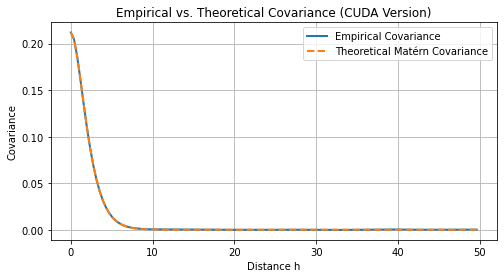
\includegraphics[width=0.5\linewidth]{pics/1D_Empirical_vs_Theoretical_Covariance_2048_100.0_2_1.png}
    \caption{1D stationary covariance function}
    \label{1d_matern_covariance}
\end{figure}

\subsection{1D random fields}
Here are some examples of 1D random fields computed by classical methods in Fig \ref{1drf}.
\begin{figure}[H]
    \centering
\begin{minipage}[t]{0.3\textwidth}  % 宽度可自定义,例如 0.45\textwidth
    \centering
    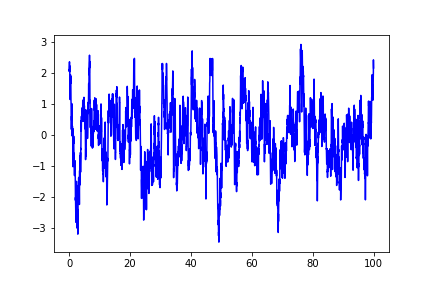
\includegraphics[width=\textwidth]{./pics/1D_RF_4096_100.0_0.5_1.png}  % 图片路径及格式
    \caption*{$\nu = 0.5, \kappa = 1$}
  \end{minipage}
  \begin{minipage}[t]{0.3\textwidth} 
    \centering
    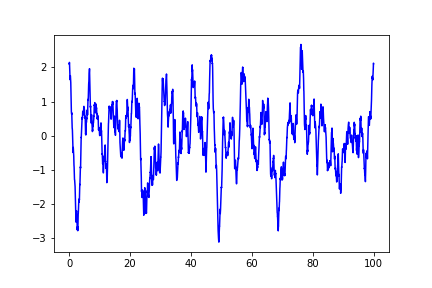
\includegraphics[width=\textwidth]{./pics/1D_RF_4096_100.0_1_1.png} 
    \caption*{$\nu = 1, \kappa = 1$}
    % \label{polymesh}
  \end{minipage}
  \begin{minipage}[t]{0.3\textwidth}
    \centering
    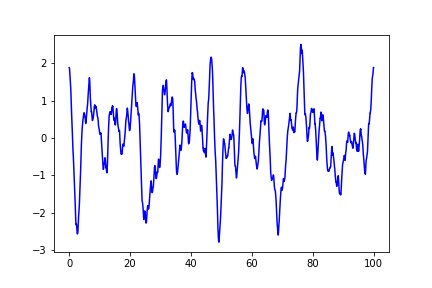
\includegraphics[width=\textwidth]{./pics/1D_RF_4096_100.0_1.5_1.png}  % 图片路径及格式
    \caption*{$\nu = 1.5, \kappa = 1$}
    % \label{prediction}
  \end{minipage}

\begin{minipage}[t]{0.3\textwidth}  % 宽度可自定义,例如 0.45\textwidth
    \centering
    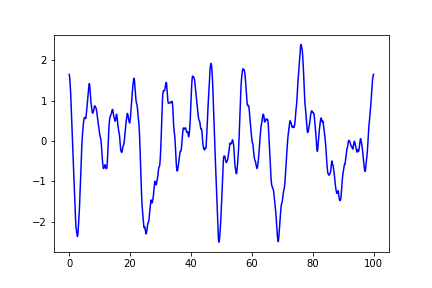
\includegraphics[width=\textwidth]{./pics/1D_RF_4096_100.0_2_1.png}  % 图片路径及格式
    \caption*{$\nu = 2, \kappa = 1$}
  \end{minipage}
  \begin{minipage}[t]{0.3\textwidth} 
    \centering
    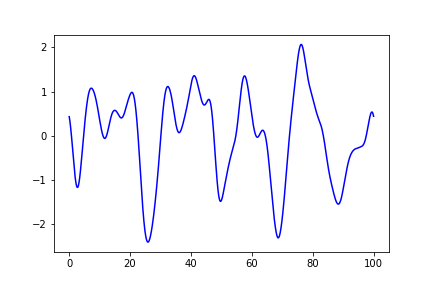
\includegraphics[width=\textwidth]{./pics/1D_RF_4096_100.0_6_1.png} 
    \caption*{$\nu = 6, \kappa = 1$}
    % \label{polymesh}
  \end{minipage}
  \begin{minipage}[t]{0.3\textwidth}
    \centering
    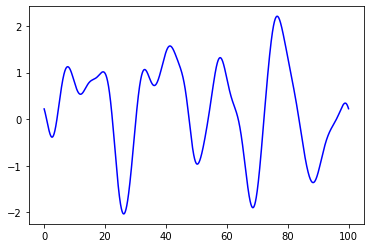
\includegraphics[width=\textwidth]{./pics/1D_RF_4096_100.0_10_1.png}  % 图片路径及格式
    \caption*{$\nu = 10, \kappa = 1$}
    % \label{prediction}
  \end{minipage}

    \caption{1D Random Field (Normalized)}
    \label{1drf}
\end{figure}

Use MLP to learn the spectral density of the random field, and then generate the random field by inverse Fourier transform.
\begin{figure}[H]
    \centering
\begin{minipage}[t]{0.3\textwidth}  % 宽度可自定义,例如 0.45\textwidth
    \centering
    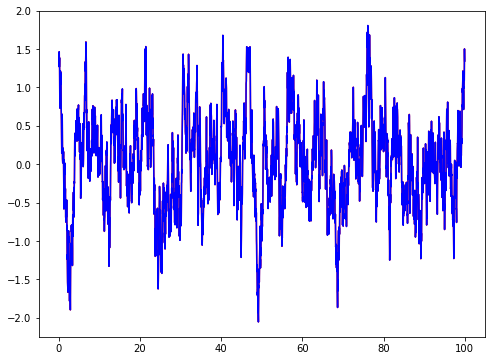
\includegraphics[width=\textwidth]{./pics/1D_NeuralRF_4096_100.0_0.5_1.png}  % 图片路径及格式
    \caption*{$\nu = 0.5, \kappa = 1$}
  \end{minipage}
  \begin{minipage}[t]{0.3\textwidth} 
    \centering
    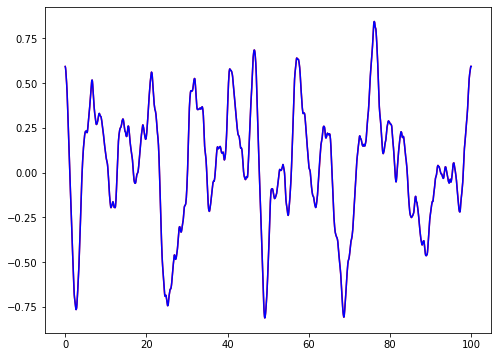
\includegraphics[width=\textwidth]{./pics/1D_NeuralRF_4096_100.0_2_1.png} 
    \caption*{$\nu = 2, \kappa = 1$}
    % \label{polymesh}
  \end{minipage}
  \begin{minipage}[t]{0.3\textwidth}
    \centering
    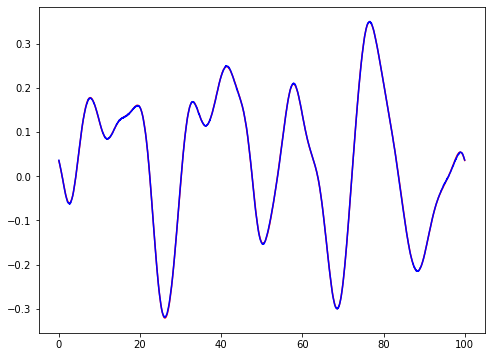
\includegraphics[width=\textwidth]{./pics/1D_NeuralRF_4096_100.0_10_1.png}  % 图片路径及格式
    \caption*{$\nu = 10, \kappa = 1$}
    % \label{prediction}
  \end{minipage}

    \caption{1D Neural Random Field}
    \label{1dnrf}
\end{figure}


Assume discrete samples of the stochastic simulator $\mathcal{M}(x, \omega)$ are given as:
\begin{equation}
	\mathcal{T}_r :=\left\{\left(x_i^r, \mathcal{M}(x_i^r, \omega^r)\right): i=1,2,\cdots,N^r\right\}, \quad r=1,2,\cdots,R.
\end{equation}
in the form of discrete evaluations of the stochastic simulator on R trajectories, where for
every r, $\{x_i^r\}_{i=1}^{N^r}$ is an i.i.d. sample from the input distribution $\mu$, and $\mathcal{M}(x_i^r, \omega^r)$ is the output of the stochastic simulator.
Here we assume for notational simplicity that $N^r = N$ for all $r$.

That is we have $R$ samples $u(x)$. By the definition of spectral density, we can have the estimation of $S_u(k)$:
\begin{equation}
    S_u(k) = \frac{1}{(2\pi)^d}\frac{1}{R}\sum_{r=1}^R\left(\left\|(\mathcal{F}u_r)(k)\right\|^2\right)
\end{equation}
For the above example, the solution can be rewritten as:
\begin{equation}
    u(x) = \mathcal{F}^{-1}\left[\hat{W}(k)(S_u(k))^{1/2}\right](x)
\end{equation}

\begin{figure}[H]
    \centering
    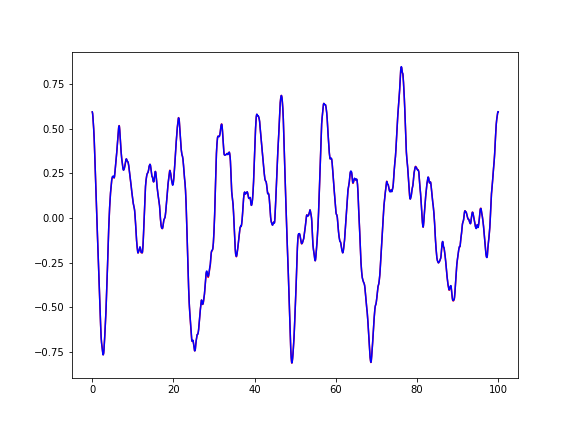
\includegraphics[width=0.5\linewidth]{pics/1D_DataDrivenRF_4096_100.0_2_1.png}
    \caption{1D Data-Driven Random Field}
    \label{DataDrivenRF}
\end{figure}



\subsection{2D random fields}
2D is similar. Neural 2D random field is vertified.
\begin{figure}[H]
    \centering
\begin{minipage}[t]{0.3\textwidth}  % 宽度可自定义,例如 0.45\textwidth
    \centering
    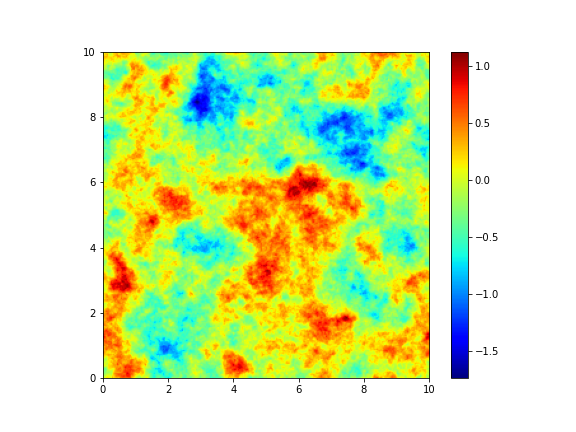
\includegraphics[width=\textwidth]{./pics/2D_RF_256_10.0_0.5_1.png}  % 图片路径及格式
    \caption*{$\nu=0.5, \kappa=1$}
  \end{minipage}
  \begin{minipage}[t]{0.3\textwidth} 
    \centering
    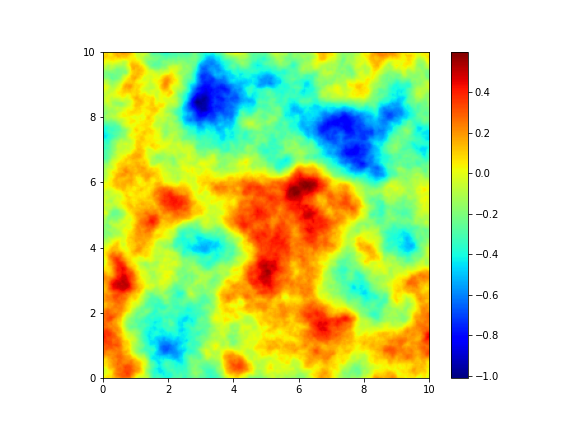
\includegraphics[width=\textwidth]{./pics/2D_RF_256_10.0_1_1.png} 
    \caption*{$\nu=1, \kappa=1$}
    % \label{polymesh}
  \end{minipage}
  \begin{minipage}[t]{0.3\textwidth}
    \centering
    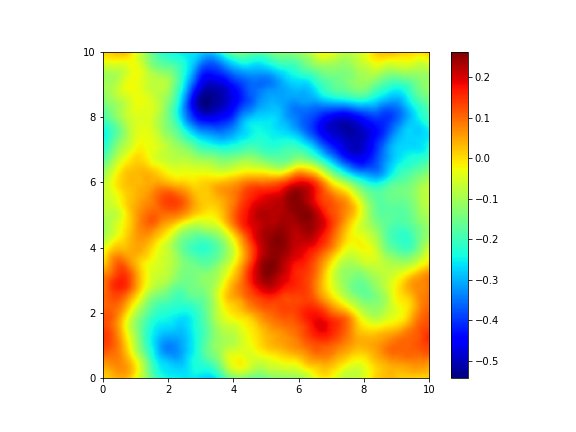
\includegraphics[width=\textwidth]{./pics/2D_RF_256_10.0_2_1.png}  % 图片路径及格式
    \caption*{$\nu=2, \kappa=1$}
    % \label{prediction}
  \end{minipage}

\begin{minipage}[t]{0.3\textwidth}  % 宽度可自定义,例如 0.45\textwidth
    \centering
    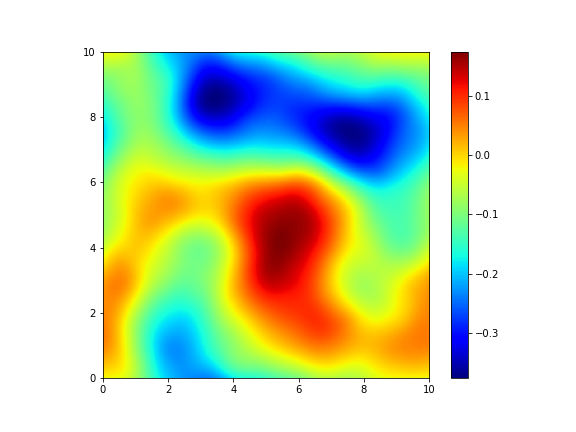
\includegraphics[width=\textwidth]{./pics/2D_RF_256_10.0_3_1.png}  % 图片路径及格式
    \caption*{$\nu=3, \kappa=1$}
  \end{minipage}
  \begin{minipage}[t]{0.3\textwidth} 
    \centering
    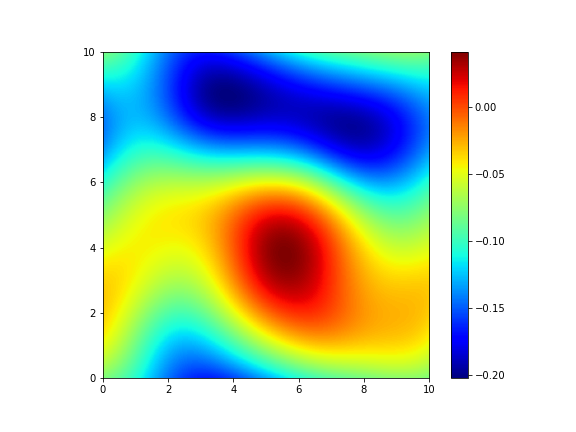
\includegraphics[width=\textwidth]{./pics/2D_RF_256_10.0_6_1.png} 
    \caption*{$\nu=6, \kappa=1$}
    % \label{polymesh}
  \end{minipage}
  \begin{minipage}[t]{0.3\textwidth}
    \centering
    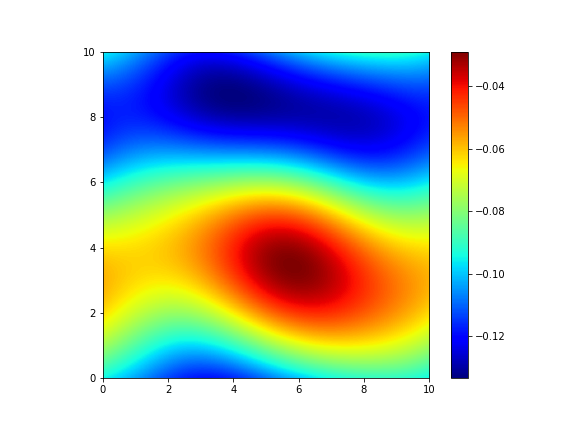
\includegraphics[width=\textwidth]{./pics/2D_RF_256_10.0_10_1.png}  % 图片路径及格式
    \caption*{$\nu=10, \kappa=1$}
    % \label{prediction}
  \end{minipage}

    \caption{2D Random Field}
    \label{2drf}
\end{figure}

\begin{figure}[H]
    \centering
\begin{minipage}[t]{0.3\textwidth}  % 宽度可自定义,例如 0.45\textwidth
    \centering
    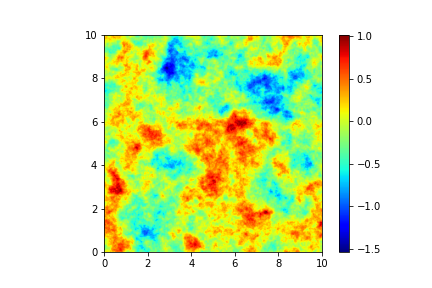
\includegraphics[width=\textwidth]{./pics/2D_NeuralRF_256_10.0_0.5_1.png}  % 图片路径及格式
    \caption*{$\nu=0.5, \kappa=1$}
  \end{minipage}
  \begin{minipage}[t]{0.3\textwidth} 
    \centering
    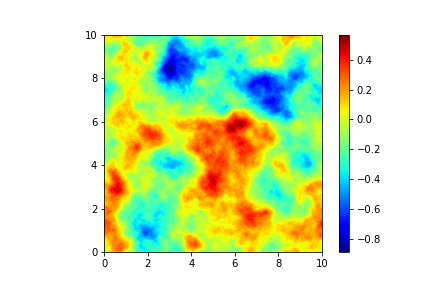
\includegraphics[width=\textwidth]{./pics/2D_NeuralRF_256_10.0_1_1.png} 
    \caption*{$\nu=1, \kappa=1$}
    % \label{polymesh}
  \end{minipage}
  \begin{minipage}[t]{0.3\textwidth}
    \centering
    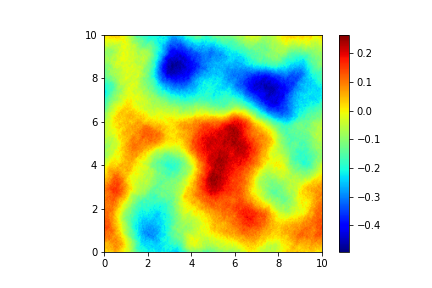
\includegraphics[width=\textwidth]{./pics/2D_NeuralRF_256_10.0_2_1.png}  % 图片路径及格式
    \caption*{$\nu=2, \kappa=1$}
    % \label{prediction}
  \end{minipage}

\begin{minipage}[t]{0.3\textwidth}  % 宽度可自定义,例如 0.45\textwidth
    \centering
    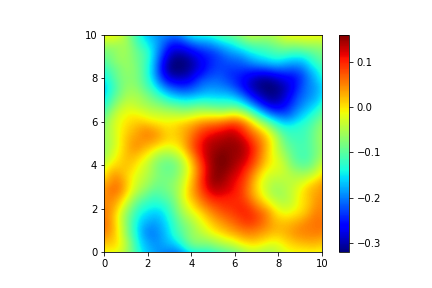
\includegraphics[width=\textwidth]{./pics/2D_NeuralRF_256_10.0_3_1.png}  % 图片路径及格式
    \caption*{$\nu=3, \kappa=1$}
  \end{minipage}
  \begin{minipage}[t]{0.3\textwidth} 
    \centering
    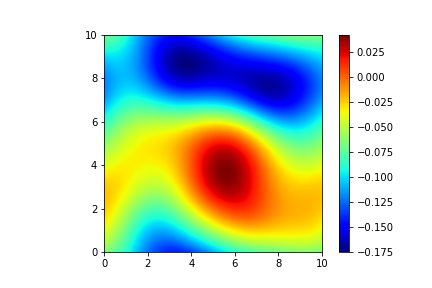
\includegraphics[width=\textwidth]{./pics/2D_NeuralRF_256_10.0_6_1.png} 
    \caption*{$\nu=6, \kappa=1$}
    % \label{polymesh}
  \end{minipage}
  \begin{minipage}[t]{0.3\textwidth}
    \centering
    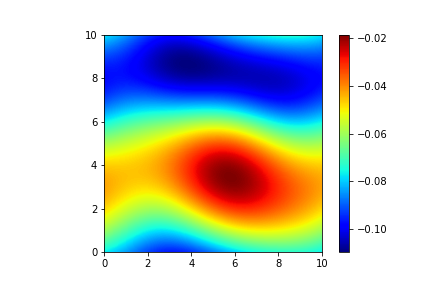
\includegraphics[width=\textwidth]{./pics/2D_NeuralRF_256_10.0_10_1.png}  % 图片路径及格式
    \caption*{$\nu=10, \kappa=1$}
    % \label{prediction}
  \end{minipage}

    \caption{2D Neural Random Field}
    \label{2dnrf}
\end{figure}



\section{Conclusion}
Q1: For general SPDE, given the equation, how to simulate the random field? 
Or inversely, given the random field data, how to infer the equation?

Q2: What is the relationship between the equation and the covariance function? 
For $\forall \mathcal{M}(x, \omega)$, can we find a differential operator $\mathcal{L}$ and a noise $\mathcal{W}$ s.t. $\mathcal{L}\mathcal{M} =\mathcal{W}$?

Q3: Generally speaking, given the covariance function of $\mathcal{M}(x, \omega)$, 
how can we simulate the random field with DNN?

Consider:
\begin{itemize}
	\item Generative Model: GAN, VAE, Flow-based model
	\item Neural Operator: DeepONet, FNO, etc.
\end{itemize}

\newpage
\bibliographystyle{unsrt}
\bibliography{references}

\newpage
\appendix
\section{Fourier Transform}\label{FourierTransform}
\begin{definition}
	Define the Fourier transform of $u(x)$ as:
	\begin{equation}\left\{
		\begin{aligned}
			& \mathcal{F}u(k) = \int_{\mathbb{R}^d} u(x) e^{-ikx} dx,\\
			& \mathcal{F}^{-1}u(x) = \frac{1}{(2\pi)^{d}}\int_{\mathbb{R}^d} u(k) e^{ikx} dk.
		\end{aligned}\right.
	\end{equation}
\end{definition}
\section{Polynomial Chaos Expansion}\label{PCE}
A spectral expansion in $L_{\mu}(D)$ is called chasos expansion. By defining the inner product in $L_{\mu}(D)$ as:
\begin{equation}
	\langle f, g \rangle_{\mu} = \int_D f(x) g(x) d\mu(x),
\end{equation}
the space of $L_\mu(D)$ is a Hilbert space.
\begin{theorem}
	Let $\{\phi_i(x)\}_{i=1}^{\infty}$ be an orthonormal basis of $L_\mu(D)$, i.e.
	\begin{equation}
		\begin{aligned}
			&1. \int_D \phi_i(x) \phi_j(x) d\mu(x) = \delta_{ij},\\
			&2. {\phi_i(x)} \text{ is dense in } L_\mu(D).
		\end{aligned}
	\end{equation}
	Then the chasos expansion of $\mathcal{M}(x, \omega)\in L_\mu(D)$ is given by:
	\begin{equation}
		\mathcal{M}(x, \omega) = \sum_{i=1}^{\infty} c_i \phi_i(x),
	\end{equation}
	where $c_i(x)=\langle \mathcal{M}, \phi_i\rangle_{\mu}$ are the coefficients of the expansion.
\end{theorem}
	

\section{Karhunen-Loeve Expansion}\label{KLE}
Let $\mu(x)$ be the mean function and $C(x, y)$ be the covariance function of $\mathcal{M}(x, \omega)$. 
Assume that $D$ is bounded, $C(x, y)$ is continuous and $\mathcal{M}(x, \cdot)$ has finite variables for all $x\in D$.


\begin{theorem}\label{KL-expansion}
    The Karhunen-Loeve expansion of $\mathcal{M}(x, \omega)$ is given by:
    \begin{equation}
        \mathcal{M}(x, \omega) = \mu(x) + \sum_{i=1}^{\infty} \lambda_i \phi_i(x) \xi_i(\omega),
    \end{equation}
	where $\lambda_i$ and $\phi_i(x)$ are the eigenvalues and eigenfunctions of the covariance operator $\mathcal{C}$:
\begin{equation}
	(\mathcal{C}\phi_i)(x) =\int_D Cov(\mathcal{M}(x, \omega), \mathcal{M}(y, \omega)) \phi_i(y) dy= \int_D C(x, y) \phi_i(y) dy = \lambda_i \phi_i(x).
\end{equation}
where $C(x,y), x,y\in D$ is the covariance function of $\mathcal{M}(x, \omega)$. The KL-random variables $\xi_i(\omega)$ are the result of the projection of $\mathcal{M}(x, \omega)$ onto the eigenfunctions $\phi_i(x)$:
\begin{equation}
	\xi_i(\omega) = \frac{1}{\sqrt{\lambda_i}}\int_D (\mathcal{M}(x, \omega)-\mu(x)) \phi_i(x) dx.
\end{equation}
\end{theorem}
Note that both $\{\phi_i(x)\}_{i=1}^{\infty}$ and $\{\xi_i(\omega)\}_{i=1}^{\infty}$ are orthonormal bases, 
one capturing the “spatial” variation  of $\mathcal{M}(x, \omega)$ over $D$ (in terms of $x$), 
the other capturing the stochastic variation of $\mathcal{M}(x, \omega)$ (in terms of $\omega$).

\begin{theorem}[Mercer's theorem]
	The covariance function $C(x, y)$ of $\mathcal{M}(x, \omega)$ can be expressed as:
\begin{equation}
	C(x, y) = \sum_{i=1}^{\infty} \lambda_i \phi_i(x) \phi_i(y).
\end{equation}
It follows that the average variance of the random field over the domain $D$ is equal to $\sum_{i=1}^{\infty} \lambda_i$.
\end{theorem}

In most cases, the integral eigenvalue problem in Equ (\ref{KL-expansion}) is difficult: analytically solved and high-dimensional.

\section{Some proofs}
\begin{proof}[Proof of Thm \ref{thmtraceclass}]
\begin{equation}
  \begin{aligned}
    \mathbb{E}\left[\|u(x, \omega)\|^2_H\right] &= \mathbb{E} \left[\sum_{i=1}^\infty \langle u, \phi_i\rangle_H^2\right]\\
    &= \sum_{i=1}^\infty \mathbb{E} \left[\langle u, \phi_i\rangle_H^2\right]\\
    &= \sum_{i=1}^\infty \langle \mathcal{C}_u  \phi_i, \phi_i\rangle_H= \sum_{i=1}^\infty \lambda_i
  \end{aligned}
\end{equation}
\end{proof}

\begin{proof}[Proof of Thm \ref{spectral_density_random_field}]
    \begin{equation}
    \begin{aligned}
      S_u(k)&=\left(\mathcal{F}c\right)(k)= \int_{\mathbb{R}^d} e^{-ik h}c(h) dh\\
      &= \int_{\mathbb{R}^d} e^{-ik(x+h - x)}\mathbb{E}\left[u(x+h)u(x)\right] dh\\
      &= \mathbb{E}\left[\int_{\mathbb{R}^d} e^{-ik(x+h)}u(x+h)e^{ikx}u(x) dh\right]\\
      &= \frac{1}{(2\pi)^{d}}\mathbb{E}\left[\left|(\mathcal{F}u)(k)\right|^2\right]
    \end{aligned}
  \end{equation}
\end{proof}

\begin{proof}[Proof of Thm \ref{spectral_solution_matern}]
	Do Fourier transform on Equ (\ref{SPDE}):
\begin{equation}
	\left\{\mathcal{F}(\kappa^2 - \Delta)^{\alpha/2} u\right\}(k) = (\kappa^2 + \|k\|^2)^{\alpha/2}(\mathcal{F}u)(k)
\end{equation}
then we have 
% , and the marginal variance is
% \begin{equation}
% 	\sigma^2 = \frac{\Gamma(\nu)}{\Gamma(\nu+d/2) \kappa^{2\nu} (4\pi)^{d/2}}.
% \end{equation}
\begin{equation}\label{spectralsolution}
	(\mathcal{F}u)(k) = \hat{u}(k) = \frac{\hat{W}(k)}{(\kappa^2 + \|k\|^2)^{\alpha/2}} 
\end{equation}
Therefore, u can be written as:
\begin{equation}
	u(x) = \mathcal{F}^{-1}\left[\frac{\hat{W}(k)}{(\kappa^2 + \|k\|^2)^{\alpha/2}}\right]
\end{equation}
Then the stationary covariance function of u is given by:
\begin{equation}
	c(x) = Cov(u(x), u(0))
\end{equation}
By the definition of spectral density Equ (\ref{spectraldensity}) and Equ (\ref{spectralsolution}) we have:
\begin{equation}\label{Suk}
		S_u(k) = \frac{1}{(2\pi)^{d}}\frac{\mathbb{E}\left[\left|\hat{W}(k)\right|^2\right]}{(\kappa^2 + \|k\|^2)^{\alpha}} 
		= \frac{1}{(\kappa^2 + \|k\|^2)^{\alpha}} 
\end{equation}
Then we have the variance of u:
\begin{equation}
	c(0) = \frac{1}{(2\pi)^{d}}\int_{\mathbb{R}^d} S_u(k) dk = \frac{\Gamma(\nu)}{(4\pi)^{d/2}\kappa^{2\nu}\Gamma(\alpha) }:=\sigma^2
\end{equation}
	By Wiener-Khinchin theorem, we have:
\begin{equation}
	\begin{aligned}
		c(x) &= (\mathcal{F}^{-1}S_u)(x)=\mathcal{F}^{-1}\left[\frac{1}{(\kappa^2 + \|k\|^2)^{\alpha}}\right]\\
		&= \frac{\|x\|^\nu K_{\nu}(\kappa\|x\|)}{(4\pi)^{d/2}2^{\nu-1}\kappa^{\nu}\Gamma(\alpha)}\\
		& = \frac{\sigma^2}{2^{\nu -1}\Gamma(\nu)}(\kappa \|x\|)^\nu K_\nu (\kappa \|x\|)
	\end{aligned}
\end{equation}
\end{proof}
\begin{remark}
	To make $c(0) = 1$, we can multiple a constant factor $\sigma_1$ to $S_u(k)$:
	\begin{equation}
		\sigma_1^2 = \frac{\Gamma(\alpha) \kappa^{2\nu}(4\pi)^{d/2}}{\Gamma(\nu)}
	\end{equation}
	Then the corresponding function of u is:
	\begin{equation}
		u(x) = \mathcal{F}^{-1}\left[\frac{\sigma_1\hat{W}(k)}{(\kappa^2 + \|k\|^2)^{\alpha/2}}\right]
	\end{equation}
\end{remark}


\end{document}